% !TEX program = pdflatex
\documentclass{article}
\usepackage[margin=1in]{geometry}
\usepackage{amsmath,amsfonts,amssymb}
\usepackage{graphicx}
\usepackage{booktabs}
\usepackage{hyperref}
\usepackage{caption}
\usepackage{subcaption}

\title{Compression Scaling Laws for Transformer Compressors Across Modalities}
\author{Ram Bharadwaj\\Independent Researcher}
\date{July 19, 2025}

\begin{document}
\maketitle

\begin{abstract}
We report empirical scaling laws for true arithmetic-coded compression ratios (CR) of Pythia transformers (70M to 1.4B parameters, five checkpoints) on text (Enwik8), image (ImageNet patches), and speech (LibriSpeech) data. Across 75 model-checkpoint pairs per modality, CR follows
\[
  \mathrm{CR}(P,S) = a + b\,P^{-\alpha} + c\,S^{-\beta},
\]
with fitted coefficients shown in Table~\ref{tab:fits}. Exponents $(\alpha,\beta)$ align with the cross-entropy scaling laws of Kaplan et al.\ on text and vary systematically for images and audio, suggesting a bias–variance view: model size suppresses representation error ($\propto P^{-\alpha}$), training steps suppress optimization error ($\propto S^{-\beta}$). Code and data are available at \href{https://github.com/rokosbasilisk/scaling-laws-for-compression}{\texttt{rokosbasilisk/scaling-laws-for-compression}}.
\end{abstract}

\section{Introduction}
Transformer language models serve as entropy coders: the negative log probability $-\log_2\hat p_\theta(x_{t+1}\mid x_{\le t})$ equals the bit cost of arithmetic coding. Kaplan et al.~\cite{kaplan2020scaling} showed that cross-entropy scales as a power law with model size and training tokens, and Del\'etang et al.~\cite{deletang2023compression} demonstrated that LLMs compress diverse modalities with arithmetic coding. We extend these findings by fitting joint power laws in model parameter count $P$ and training steps $S$ across text, image, and speech.

\section{Methodology}
\subsection{Datasets}
We use three benchmarks, each split into 2048 equal-sized byte chunks:
\begin{itemize}\itemsep0pt
  \item \textbf{Enwik8}: first 100M bytes of Wikipedia XML.
  \item \textbf{ImageNet patches}: 2048 random 32$\times$64 grayscale crops from ILSVRC validation.
  \item \textbf{LibriSpeech chunks}: 2048 PCM segments (2048 samples at 16 kHz).
\end{itemize}

\subsection{Models and Checkpoints}
Pythia models with $P\in\{70,160,410,1000,1400\}$ million parameters and checkpoints at $S\in\{1{,}000,8{,}000,32{,}000,128{,}000,143{,}000\}$ optimization steps, totaling 25 pairs per modality.

\subsection{Compression Pipeline}
Chunks are mapped to ASCII, tokenized with Pythia’s tokenizer, and compressed via true arithmetic coding driven by token probabilities (see \texttt{code.py}). We compute CR as compressed bits divided by original bits.

\section{Results}
Figure~\ref{fig:surfaces} visualizes the measured CR surfaces and the fitted power-law models. Table~\ref{tab:fits} lists the optimized coefficients $(a,b,c,\alpha,\beta)$ for each modality.

\begin{figure}[h]
  \centering
  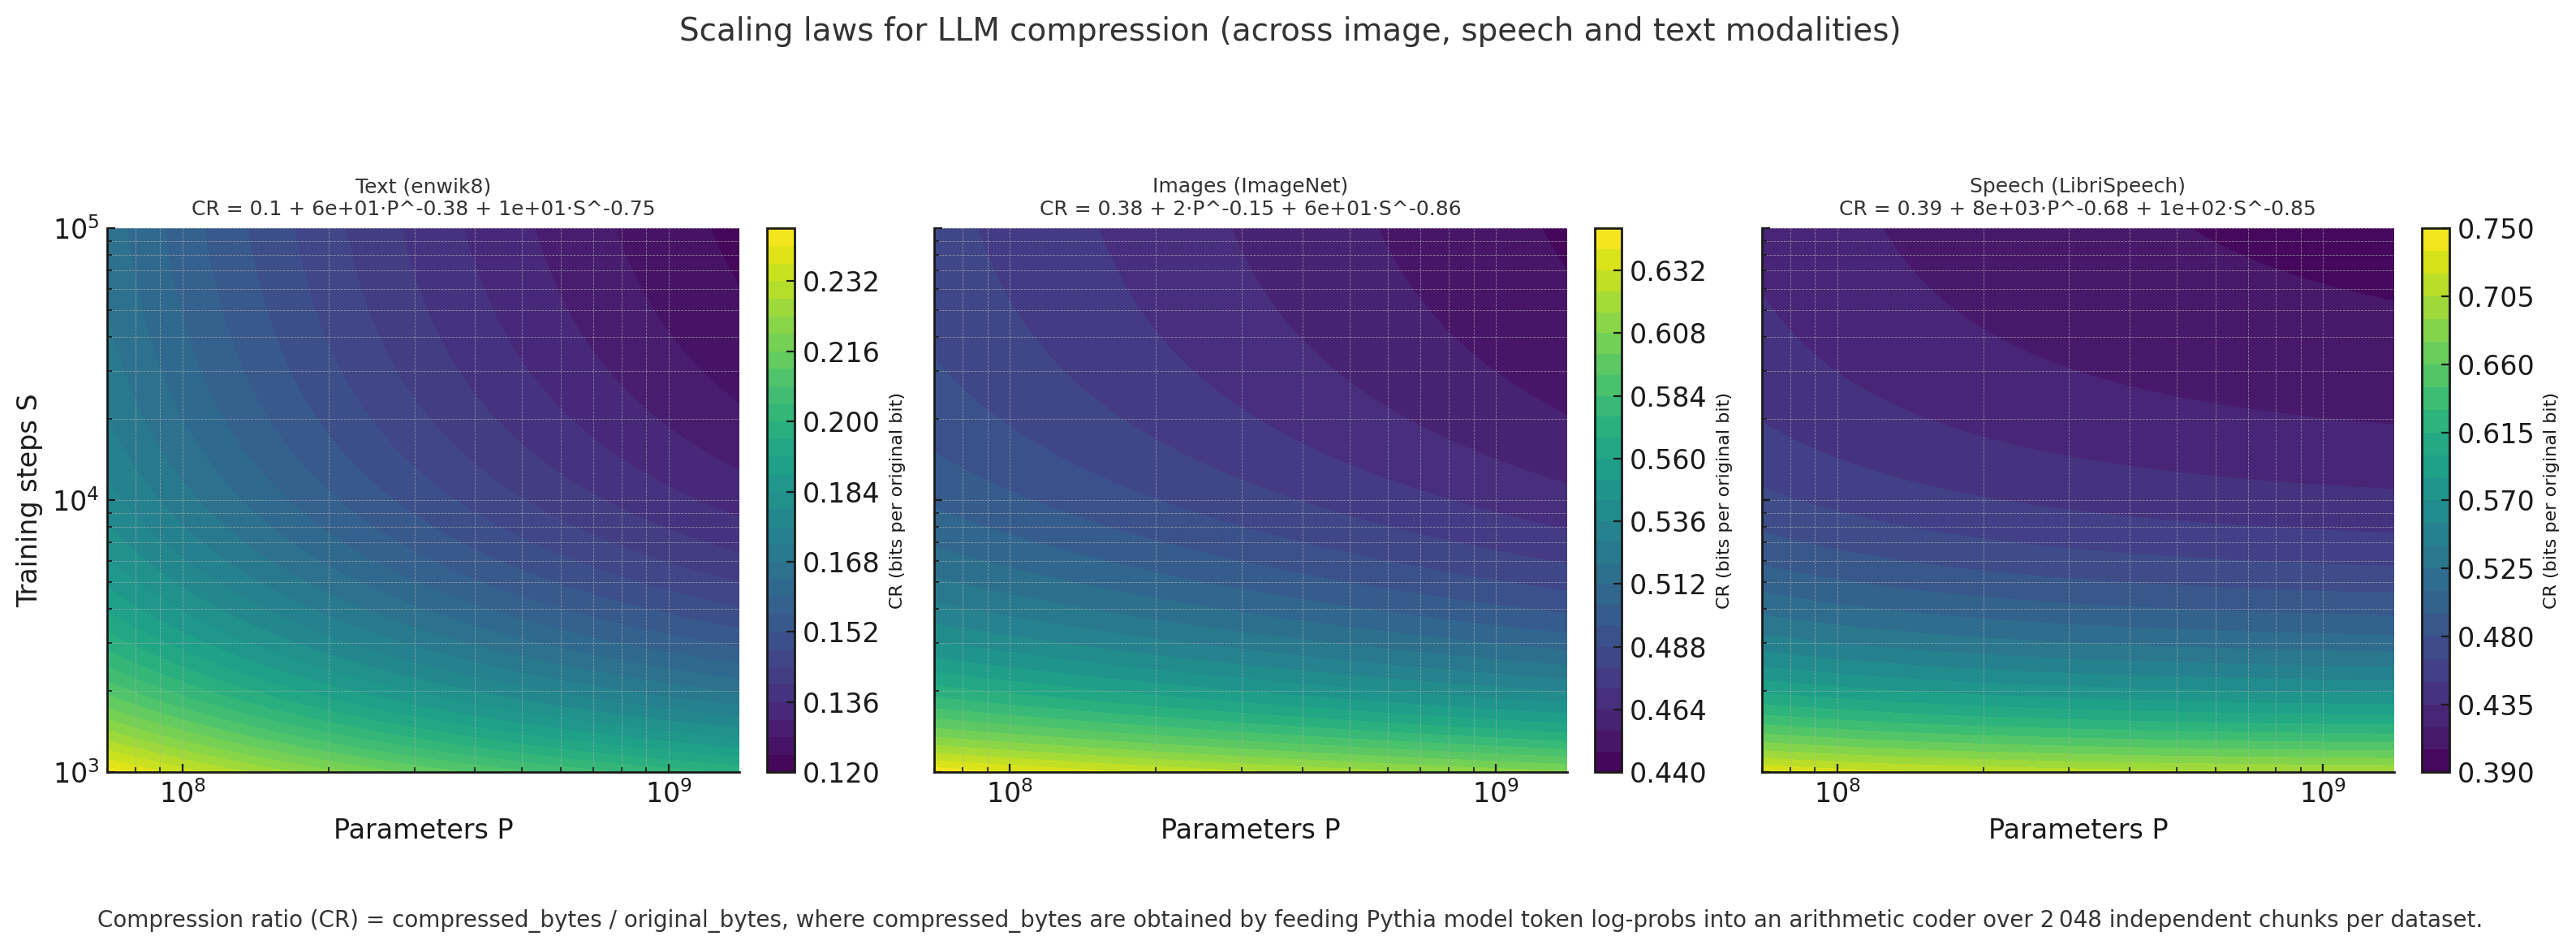
\includegraphics[width=0.8\linewidth]{scaling_laws_for_compression.png}
  \caption{Compression ratio surfaces: lower is better.}
  \label{fig:surfaces}
\end{figure}

\begin{table}[h]
  \centering
  \begin{tabular}{lrrrrr}
    \toprule
    Dataset & $a$   & $b$     & $c$   & $\alpha$ & $\beta$ \\
    \midrule
    Text (Enwik8)       & 0.10 &    60   &   10  & 0.38 & 0.75 \\
    Image (ImageNet)    & 0.38 &     2   &   60  & 0.15 & 0.86 \\
    Speech (LibriSpeech)& 0.39 & 8\,000  &  100  & 0.68 & 0.85 \\
    \bottomrule
  \end{tabular}
  \caption{Fitted coefficients for $\mathrm{CR}(P,S)=a+bP^{-\alpha}+cS^{-\beta}$.}
  \label{tab:fits}
\end{table}

\section{Discussion}
The irreducible term $a$ matches estimated dataset entropy rates. For text, $(\alpha,\beta)=(0.38,0.75)$ align with Kaplan et al.’s $(0.076,0.095)$ after converting bits/token to bytes per bit. Higher exponents for image and speech reflect increased data complexity and SGD noise. These laws inform compute-optimal allocations between $P$ and $S$ under a fixed budget.

\section{Conclusion}
We present unified scaling laws for LLM-based compression across modalities, grounded in established cross-entropy theory. Future work may extend to other architectures and explore sparsity for more efficient compression.

\begin{thebibliography}{9}
\bibitem{kaplan2020scaling}
J.~Kaplan \emph{et~al.}, 
``Scaling Laws for Neural Language Models,'' 
arXiv:2001.08361, 2020.

\bibitem{deletang2023compression}
G.~Del\'etang \emph{et~al.}, 
``Language Modeling Is Compression,'' 
arXiv:2309.10668, 2023.
\end{thebibliography}

\end{document}

